%%% Local Variables:
%%% mode: latex
%%% TeX-master: t
%%% End:

\chapter{SiO{\heiti\text{$_2$}}胶体晶体模板制备}
\label{ch:synth_PhC}

\section{引言}
作为光子晶体材料的结构来源及重要组成部分,光子晶体模板在光子晶体的制备中具有重要意义。这里我们采用胶体晶体自组装的方法来制备光子晶体模板。
由于制备本文中聚合物反蛋白石光子晶体时需要使用有机相溶剂,在胶体颗粒材料的选择上,我们选用了对有机溶剂稳定的SiO\text{$_2$}胶体颗粒来制备模板。
由于本文中涉及了平面型及球形的光子晶体材料的制备,本章中将就不同维度上的三维光子晶体模板制备进行讨论,并将所得的光子晶体模板用于其余章节的工作中。

单分散SiO\text{$_2$}胶体颗粒是制备光子晶体模板的关键组成部分。
含硅前驱体在酸碱条件下的水解能够形成光子晶体微球,而Stöber等于1968年首次提出了利用醇-水-碱体系制备含二氧化硅单分散微球的方法\cite{Stoeber1968Controlled}。
通过对Stöber方法的改进,仅利用不同组分的调节,达到对某一范围内SiO\text{$_2$}胶体颗粒粒径的调控目的。其基本原理可以见图\ref{fig:stoeber}。
\begin{figure}[htbp]
	\centering
	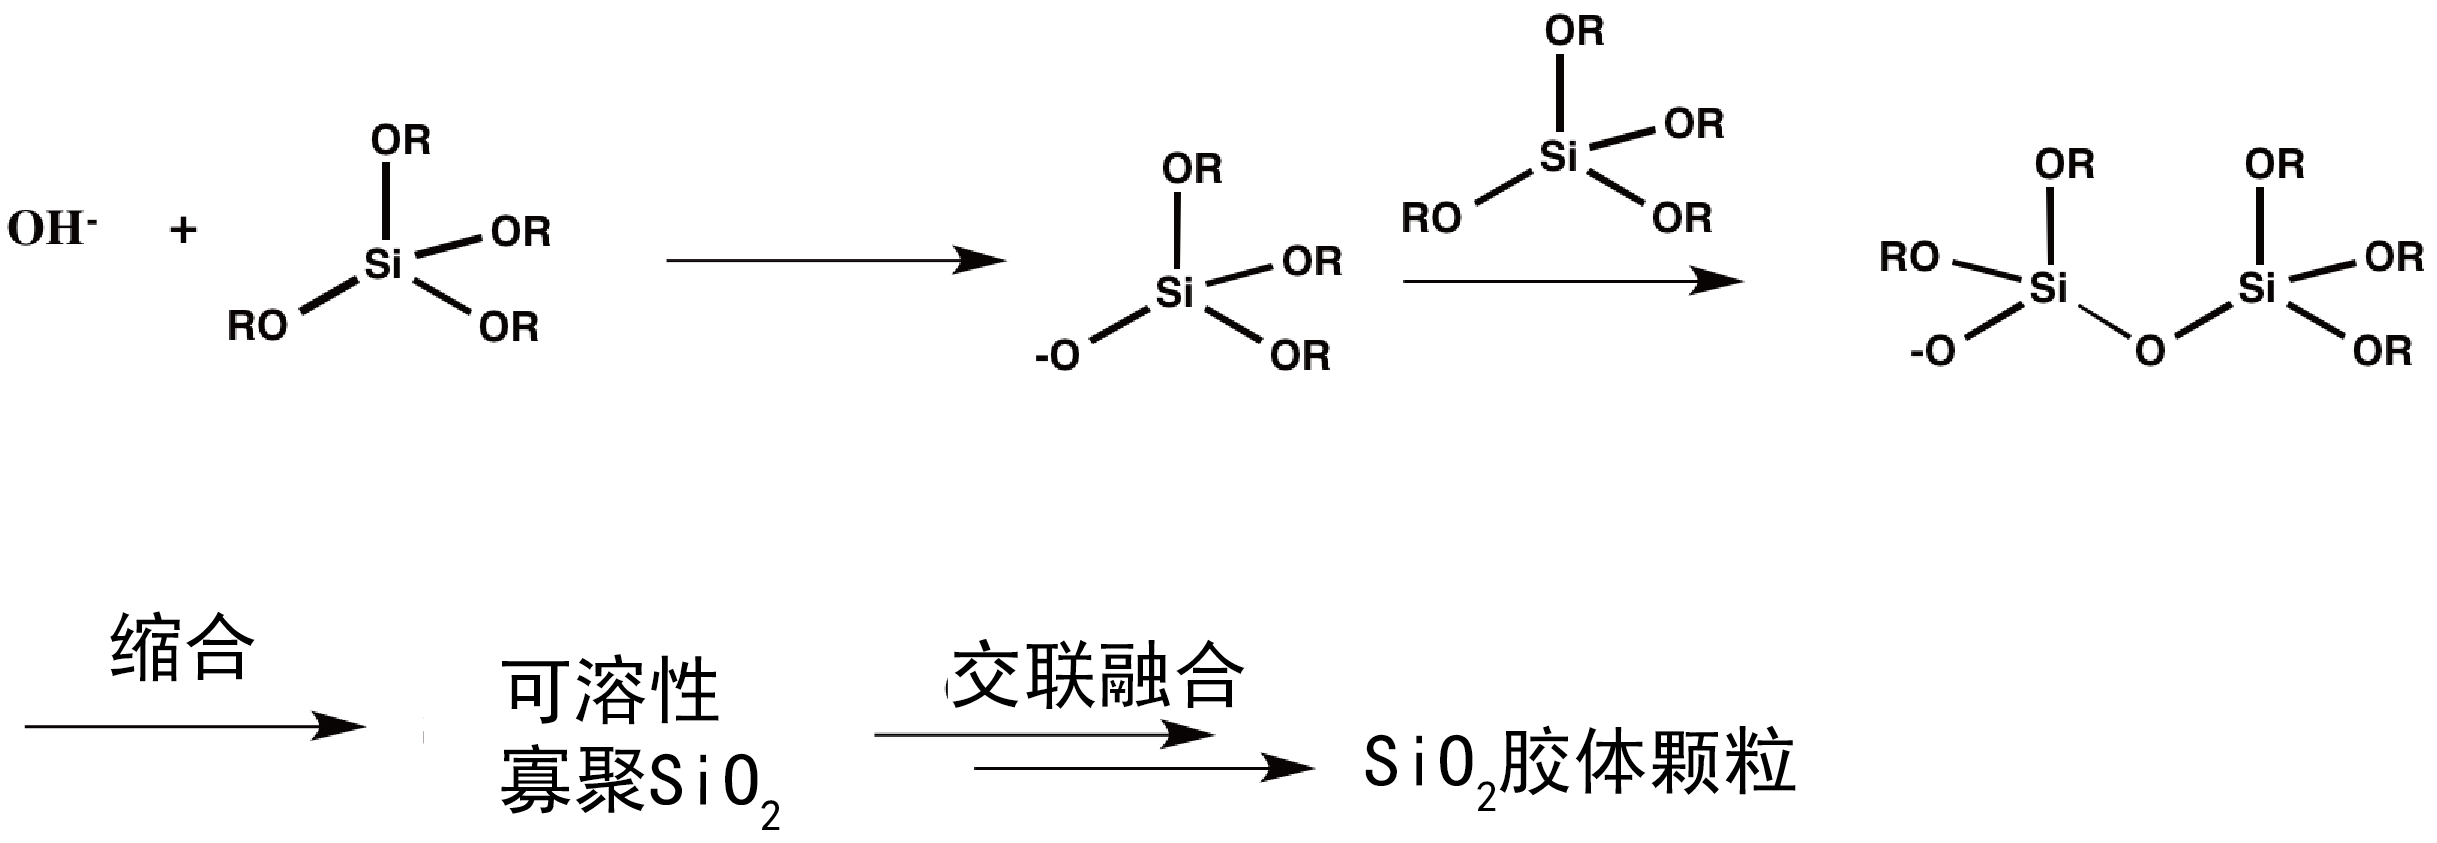
\includegraphics[width=\linewidth]{figures/ch2-stoeber.png}
	\caption{Stöber法生长的SiO\text{$_2$}胶体颗粒的原理示意图}
	\label{fig:stoeber}
\end{figure}
本章中将就不同组分调节SiO\text{$_2$}胶体颗粒粒径进行探究,并将不同尺寸的SiO\text{$_2$}胶体颗粒进行胶体晶体组装形成光子晶体模板。

在不同维度的光子晶体模板材料方面,本章中将探索三种方法生长的光子晶体材料。首先,利用溶剂挥发诱导的自组装法生长了玻璃薄片上的三维光子晶体;其次,为了制备较大面积的三维光子晶体模板,发展了一种利用单层SiO\text{$_2$}胶体颗粒逐层堆积组装(LbL)制备三维光子晶体的方法;最后,结合微流控液滴法,制备了微米至亚毫米尺度上的光子晶体微球模板。

\section{实验部分}
\subsection{实验材料与仪器}
本章中所使用的实验材料与仪器分别见表~\ref{tab:ch2-material}与~\ref{tab:ch2-instrument}。

\begin{table}[htbp]
  \centering
  \caption{本章所用实验材料}
  \label{tab:ch2-material}
    \begin{tabularx}{\linewidth}{XXXX}
      \toprule[1.5pt]
      {\heiti 药品名称} & {\heiti 纯度} & {\heiti 来源} & {\heiti 处理方法}\\
      \midrule[1pt]
      四乙氧基硅烷 & 分析纯 & 国药集团化学试剂有限公司 & 用前重蒸\\
      氨水 & 分析纯 & 国药集团化学试剂有限公司 & 直接使用\\
      无水乙醇 & 分析纯 & 国药集团化学试剂有限公司 & 直接使用\\
      甲基丙烯酸甲酯(MMA) & 98\% & Alfa Aesar & 直接使用\\
      乙二醇二甲基丙烯酸酯(EGDMA) & 98\% & Alfa Aesar & 直接使用\\
      偶氮二异丁腈(AIBN) & 98\% & Alfa Aesar & 重结晶\\
      氢氟酸(HF) & w/w\%=40\% & Acros & 直接使用\\
      去离子水 & 分析纯 & 自制 & 直接使用\\
      \bottomrule[1.5pt]
    \end{tabularx}
\end{table}

\begin{table}[htbp]
  \centering
  \caption{本章所用仪器}
  \label{tab:ch2-instrument}
    \begin{tabularx}{\linewidth}{XXX}
      \toprule[1.5pt]
      {\heiti 仪器名称} & {\heiti 仪器型号} & {\heiti 厂家} \\
      \midrule[1pt]
      量筒 & 10ml、25ml、100ml & 北京玻璃厂 \\
      圆底烧瓶 & 250ml & Synthware\\
      Eppendorf移液器 & 5ml & 大龙科技\\
      台式离心机 & TDL-60B &上海亚荣\\
      磁力搅拌器 & HS-7 & 大龙科技\\
      水浴超声仪 & SCQ-H600A & 松江超声 \\
      反射光纤光谱仪 & USB2000 & OceanOptics\\
      场发射扫描电子显微镜(SEM) & LEO-1503 & Bruker\\
      \bottomrule[1.5pt]
    \end{tabularx}
\end{table}

\subsection{Stöber法生长SiO\text{$_2$}胶体颗粒的探究}

本文中利用改进的Stöber法生长单分散的SiO\text{$_2$}胶体颗粒。其方法如下:

1. A液:将一定体积的去离子水、氨水及无水乙醇加入圆底烧瓶中,并用磁力搅拌器维持约500 rpm速度,在30 $^{\circ}$C油浴环境中均匀搅拌。

2. B液:将一定体积的TEOS、无水乙醇加入另一个烧瓶并混合。A液与B液的总体积(不考虑溶剂混合收缩效应)之和固定为100 ml。

3. 用干净的移液器移取B液快速加入A液中混合,避免液滴沾附在瓶壁或产生大量气泡。

4. 当AB液混合完成后,将磁力搅拌速度加快至1200 rpm以使初期快速成核充分。维持油浴环境温度。混合液随其中水与氨水含量的变化,在2-30 min之内由澄清逐渐转变为乳白色悬浊液。当反应时间达到12h后终止反应。

5.将SiO\text{$_2$}胶体颗粒悬浊液置于7 ml离心管中,设定离心转速5000-7000 rpm,离心时间5min将SiO\text{$_2$}胶体颗粒离心至管底部。弃置上上清液并将固体固体重新超声分散在乙醇中。将SiO\text{$_2$}洗涤5次,直到上清液呈现中性。

6.将洗涤过SiO\text{$_2$}胶体颗粒离心后置于60 $^{\circ}$C烘箱中干燥5h,将固体粉末在研钵中充分研磨,以备于后续表征与胶体晶体生长。

为了表征合成的SiO\text{$_2$}胶体颗粒的粒径分散性,我们将少量SiO\text{$_2$}粉末在乙醇中超声分散,并滴于干净玻璃片上进行扫描显微观察。

由Stöber法的机理\cite{Stoeber1968Controlled}可知,SiO\text{$_2$}的生长速率主要与混合液中NH\text{$_3$}及水的浓度相关,而其粒径主要与NH\text{$_3$}浓度相关,而与TEOS及乙醇的量变化不明显。
因此这里我们简化变量,固定TEOS含量,调节NH\text{$_3$}与水的含量,并同时调节乙醇的量以将溶液总体积固定为100 ml。
具体的实验参数调节如表~\ref{tab:stoeber-param}所示。其中,各溶剂的体积为其总体积, \text{$\bar r$}为SEM观察的SiO\text{$_2$}胶体颗粒平均粒径。与其对应的SEM照片见于图~\ref{fig:stober_size}。A液与B液体积分别为50ml,而A液与B液中乙醇的体积分别按其他溶剂量平衡得到。

\begin{table}[htbp]
  \centering
  \caption{Stöber法合成SiO\text{$_2$}胶体颗粒参数调节}
  \label{tab:stoeber-param}
    \begin{tabularx}{\linewidth}{XXXXXX}
      \toprule[1.5pt]
      {\heiti 序号} & {\heiti EtOH/ml} & {\heiti TEOS/ml} & {\heiti 氨水/ml} & {\heiti H{$_2$}O/ml} & {\heiti \text{$\bar r$}/nm}\\
      \midrule[1pt]
       A & 84.3 & 4.5 & 9    & 2.2 & 180 \\
       B & 84.3 & 4.5 & 9.5  & 1.7 & 200 \\
       C & 84.1 & 4.5 & 10   & 1.4 & 230 \\
       D & 83.9 & 4.5 & 10.5 & 1.1 & 270 \\
       E & 83.8 & 4.5 & 11   & 0.7 & 300 \\
       F & 83.5 & 4.5 & 12   & 0   & 330 \\
      \bottomrule[1.5pt]
    \end{tabularx}
\end{table}

\begin{figure}[htbp]
	\centering
	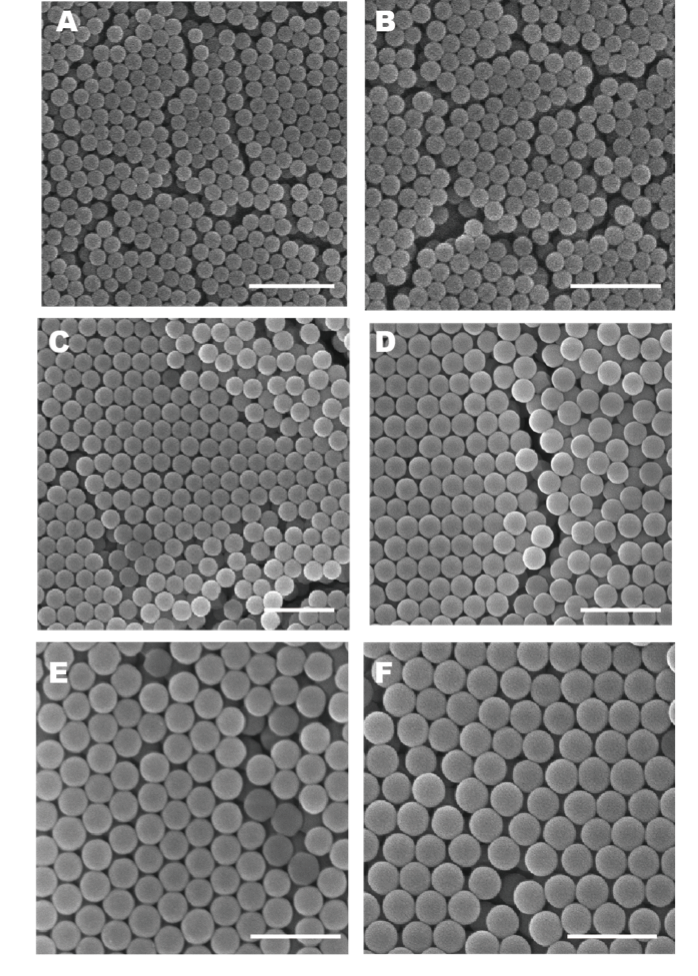
\includegraphics[width=0.8\linewidth]{figures/SEM-stober.png}
	\caption{改进的Stöber法生长SiO\text{$_2$}胶体颗粒的SEM照片,标尺均为1 \text{$\mu$}m。A-F对应与表~\ref{tab:stoeber-param}中的序号。}
	\label{fig:stober_size}
\end{figure}

由图\ref{fig:stober_size}可以看出,通过Stöber法生长的SiO\text{$_2$}胶体颗粒具有形貌规整、粒径单分散的特点。在自然溶剂蒸发条件下便能够形成一定的有序排列结构,说明这种SiO\text{$_2$}胶体颗粒可以作为光子晶体模板材料。同时,可以发现通过控制混合溶液中氨水的体积,能够对合成的SiO\text{$_2$}颗粒粒径进行调控。由公式~\ref{eqn:1-bragg}可知,用上述粒径生长的光子晶体模板的一级Bragg衍射峰落在可见光范围内,适用于裸眼观察与检测。因此,我们将采用上述粒径的SiO\text{$_2$}胶体颗粒作为原料来生长光子晶体模板。

\subsection{溶剂挥发诱导自组装制备SiO\text{$_2$}光子晶体模板}
\label{subsec:evap-template}

利用溶剂挥发诱导自组装制备SiO\text{$_2$}光子晶体模板的方法如下:

1. 将实验所用玻璃用铬酸洗液浸泡过夜,并用去离子水洗涤3次。载玻片用H\text{$_2$}SO\text{$_4$}-H\text{$_2$}O\text{$_2$}洗涤过夜,用去离子水洗涤并在氮气气氛中充分干燥。

2. 将200-300 nm的SiO\text{$_2$}粉末在无水乙醇中超声分散30 min,并用1000 rpm离心2min去除大颗粒物。余下悬浊液用乙醇调至SiO\text{$_2$}重量分数为0.3-1.0 wt\%。(每100ml Stöber生长液所合成的SiO\text{$_2$}约配至100-150 ml稀释液)。

3. 将切为1 cm\text{$\times$}4 cm的玻璃条垂直插入7 ml的西林瓶中,并在其中加入5-6 ml的上述二氧化硅乙醇分散液。

4.将上述插入玻璃片的西林瓶放置于干燥无尘的常温烘箱中,并避免震动。经过约1周至15天左右分散液中乙醇挥发完毕后,即在玻璃板上生长完成SiO\text{$_2$}光子晶体模板。

5. 将光子晶体模板在500 $^{\circ}$C的马弗炉中烧结3 h,进一步固化SiO\text{$_2$}并增强光子晶体模板的机械强度。

\begin{figure}[htbp]
  \centering
  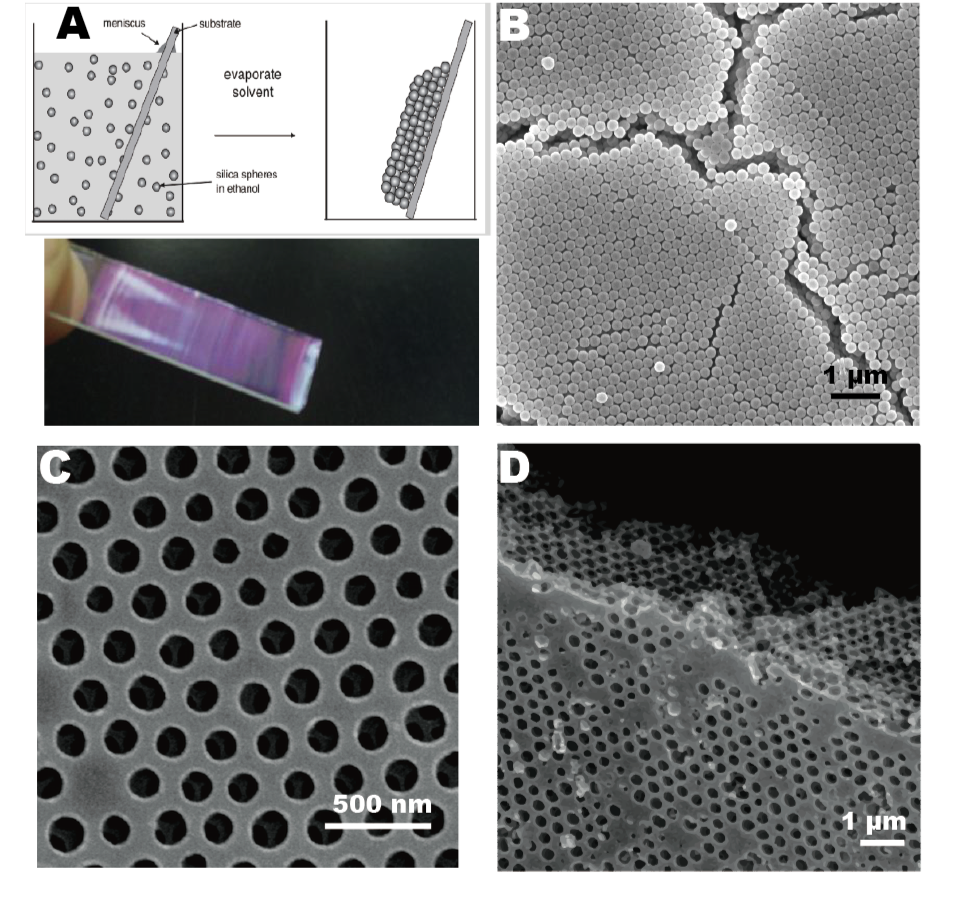
\includegraphics[width=0.8\linewidth]{figures/ch2/opal-eval.png}
  \caption{溶剂挥发诱导生长的光子晶体模板SEM照片。A. 实验原理与实物照片;B. SiO\text{$_2$}模板SEM照片;C. 反蛋白石光子晶体结构SEM正面照片;D. 反蛋白石光子晶体结构SEM侧面照片}
  \label{fig:opal-SEM}
\end{figure}

经挥发诱导自组装法生长的SiO\text{$_2$}光子晶体模板材料的实体图片见图~\ref{fig:opal-SEM}A。可以看出由胶体自组装形成的鲜艳的结构色。同时,SEM照片也显示出这种光子晶体内部的面心立方(fcc)排列结构(图~\ref{fig:opal-SEM}B),证明由溶剂挥发诱导自组装能够形成高度有序的组装结构。

同时,我们通过聚合物翻模刻蚀的方法对这种光子晶体进行了结构复制,以探究制备具有反蛋白石结构的聚合物薄膜。我们采用聚甲基丙烯酸甲酯作为示例来制备反蛋白石光子晶体。首先将0.15 g(1.76 mmol)甲基丙烯酸甲酯(MMA)、0.027 g(0.16 mmol)EGDMA 及0.005 g AIBN混合为均相溶液。
将两条有机玻璃板 (2 cm \text{$\times$} 4cm)与光子晶体模板形成三明治型复合结构,并利用毛细作用将聚合物前驱体溶液吸入光子晶体缝隙中。
当液体充分灌满时,光子晶体由于折射率变大而变为透明。将含聚合物前驱溶液的三明治结构放入80 $^{\circ}$C烘箱中,聚合12h。最后,将冷却后的光子晶体三明治结构浸泡在5\% HF溶液中,以去除复合物中的SiO\text{$_2$}胶体颗粒。通过这种方法制备的反蛋白石光子晶体结构如图~\ref{fig:opal-SEM}C、图~\ref{fig:opal-SEM}D所示,可见原结构中的fcc结构被很好地保留下来;同时,由于烧结后SiO\text{$_2$}胶体颗粒之间存在部分融合,其互补的复制后的结构具有很好的内部互穿孔道结构。
这种连续孔道结构能够很好地促进物质在反蛋白石光子晶体中的传输,并增加光子晶体的响应速率。

\subsection{逐层堆积(LbL)法制备SiO\text{$_2$}光子晶体模板}
\label{subsec:lbl-opal}

\ref{subsec:evap-template}节中使用的溶剂挥发诱导垂直沉积法制备三维光子晶体模板尽管具有较高的排列规整性,但其制备时间相当长,且制备过程中不能受到扰动,限制条件较大;这种方法所制备的光子晶体模板的大小较小,受限于挥发瓶的尺寸,且经常由于挥发不均匀导致光子晶体局部出现条纹状或块状瑕疵(图~\ref{fig:opal-SEM}A),对于制备较大面积的光子晶体模板材料具有一定的局限性。
本章中将尝试采用逐层堆积法来制备较大面积的光子晶体模板。逐层堆积法的思想是首先通过气-液界面的组装制备紧密堆积的二维光子晶体模板,并将其转移至基板上;通过多次的排列-转移过程来制备三维光子晶体模板。逐层堆积法的优点在于其制备速度较快,光子晶体模板大小可控。同时由于气-液界面组装形成的二维光子晶体厚度均一,所制备的三维光子晶体的整体完整性较高。

作为一种亲水的胶体颗粒材料,且其密度远大于水的密度,SiO\text{$_2$}胶体颗粒在水相表面组装较PS等疏水且密度较小的聚合物胶体微球更难。以往通常需要对SiO\text{$_2$}胶体颗粒表面进行疏水化处理或是在有机相溶剂表面方能实现单层组装\cite{Velikov2002LayerByLayer,Chitu2010Modified}。这些方法制备较为繁琐。Moon等利用正丁醇在水相界面上铺散的特点,发展了一种制备亲水性胶体颗粒二维组装的方法\cite{Moon2011Assembled}。这种方法同样适用于SiO\text{$_2$}的二维光子晶体制备,无须复杂的预处理过程。因此本章中将基于这种二维组装的方法,结合LbL逐层堆积法来制备SiO\text{$_2$}三维光子晶体模板材料。

利用逐层堆积(LbL)法制备SiO\text{$_2$}光子晶体模板的步骤如下:

1.将干燥粉碎后的SiO\text{$_2$}粉末配成质量分数0.1-0.4\%的正丁醇分散液,并在超声下充分分散。离心1000 rpm 2 min将不能分散的大尺寸颗粒物去除。

2. 取干净的表面皿,将切割好的玻璃片(2.5 cm \text{$\times$} 2.5 cm)置于表面皿底,并使用等离子体轰击法将玻璃片处理为亲水表面。

3. 缓慢向表面皿中加入去离子水,使得其恰好没过玻璃片表面。液面在玻璃片上方的高度不超过3 mm(以防止转移时单层胶体颗粒膜碎裂)。

4. 用细针管沿着表面皿一侧缓慢滴加1中所制备的SiO\text{$_2$}-正丁醇分散液,防止液面扰动过于剧烈。待液面完全铺散后(正丁醇分散液继续滴加无法铺散而是成为液滴滞留于表面),静置约5min使表面组装完全。用细滴管从表面皿一侧将水相吸走,直到二维光子晶体薄膜转移至玻璃片表面为止。

5. 在干净的50 $^{\circ}$C烘箱中将转移后的光子晶体膜干燥,直到光子晶体禁带颜色产生为止。

6. 重复2-5步骤,即等离子体处理-排列-转移-干燥过程,直到预定层数的三维光子晶体制备完成为止。

首先我们利用SEM来研究气液界面组装的二维光子晶体的结构特征。如图~\ref{fig:mono-SEM}A
所示,可以看出单层排列的光子晶体呈现出很好的fcc结构。
\begin{figure}[htbp]
  \centering
  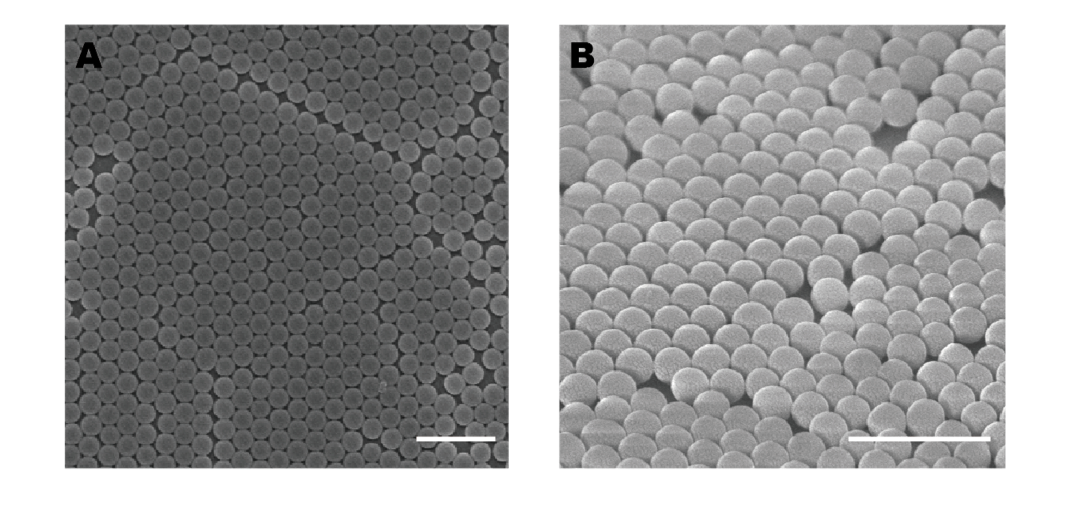
\includegraphics[width=0.8\linewidth]{figures/ch2/mono-SEM.png}
  \caption{单层排列的SiO\text{$_2$}颗粒的SEM照片。A.正面照片;B. 倾斜角度的照片。比例尺均为1 µm。}
  \label{fig:mono-SEM}
\end{figure}
倾斜角度拍摄的SEM照片图~\ref{fig:mono-SEM}B也显示这样的二维光子晶体具有单层的结构,说明利用正丁醇分散液的液相界面排列能够很好地形成单层的光子晶体结构,这也使得利用逐层堆积形成光子晶体成为可能。
同时,我们也注意到这种堆积方法非常依赖于原始SiO\text{$_2$}颗粒的单分散性。
如图~\ref{fig:mono-quality}所示,
\begin{figure}[htbp]
  \centering
  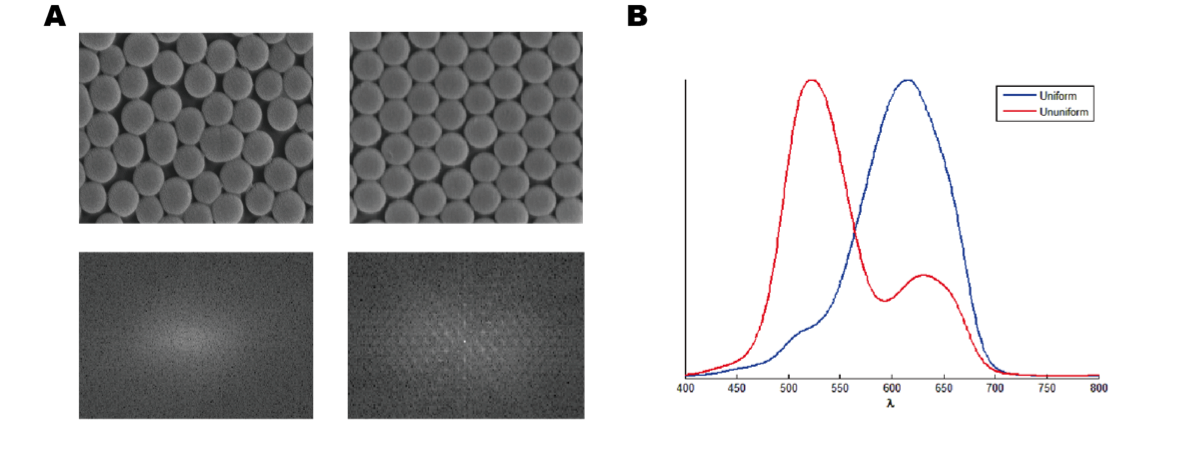
\includegraphics[width=\linewidth]{figures/ch2/mono-quality.png}
  \caption{单层排列的SiO\text{$_2$}颗粒的质量差别。A. 规整与不规整单层SiO\text{$_2$}排列的SEM照片与其对应的2D傅里叶变换结果;B. 规整与不规整的光子晶体排列的Bragg衍射峰差别。比例尺均为1 µm。}
  \label{fig:mono-quality}
\end{figure}
具有相近的平均粒径的SiO\text{$_2$}颗粒,在不同的质量下的排列有着明显的差别。当胶体微球绝大多数为球形且分散度较低时,二维光子晶体排列较好的规整性;而当光子晶体颗粒中出现较多的非球形颗粒或粒径异常的颗粒时则其组装结构规整性将会大大下降。更为具体的定量表征可以由其对应的二维傅里叶变换(2D-FFT)及Bragg衍射峰展现出来:
粒径不均匀的SiO\text{$_2$}胶体颗粒组装后的傅里叶变换图谱呈现非周期性,而粒径均一的SiO\text{$_2$}颗粒组装后傅里叶变换图显示出六方晶格特征(图~\ref{fig:mono-quality}A);同时,粒径不均一的SiO\text{$_2$}组装后的Bragg衍射峰呈现多重峰,说明其内在周期性不均一(图~\ref{fig:mono-quality}B)。
。这与此前的报道一致\cite{Jiang2001Fabrication}。因此在进行三维光子晶体制备之前需要对所使用的二氧化硅颗粒进行充分的纯化。

其次我们研究了通过逐层堆积对三维光子晶体材料质量的影响。
\begin{figure}[htbp]
  \centering
  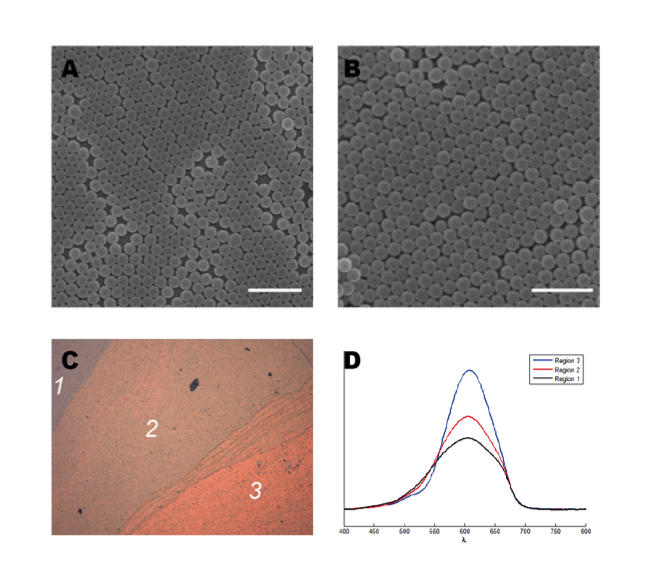
\includegraphics[width=0.95\linewidth]{figures/ch2/multilayer.png}
  \caption{单层SiO\text{$_2$}逐层堆积过程中的变化。A. 单层SiO\text{$_2$}排列的SEM图;B. 5层SiO\text{$_2$}堆积后的SEM图;C. 分别具有2层、3层、5层SiO\text{$_2$}堆积的光学照片。D. 对应与C中1-3区域的Bragg衍射峰谱图。比例尺均为1 µm。}
  \label{fig:mono-stack}
\end{figure}
如图~\ref{fig:mono-stack}所示,
随着层数的增多,光子晶体材料的组装结构的规整度具有一定的上升,fcc块区的大小也逐渐变大。这说明在逐层堆积的过程中二氧化硅微球非但没有随机排列,而是根据能量最低原则逐渐在三维尺度上堆积成为排列有序的三维光子晶体。
同时,随着层数的增加,光子晶体的Bragg衍射峰也产生变化。随着层数的增加,Bragg衍射峰的强度增大,且禁带的半峰宽逐渐变窄,表明了三维光子晶体的性质随着层数的增加而逐渐明显(图~\ref{fig:mono-stack}D)。这从原理上保证了LbL法制备三维光子晶体的可行性。

最后,我们将这种逐层堆积法制备的三维光子晶体制备了反蛋白石光子晶体,
如图~\ref{fig:mono-inverse}
。
\begin{figure}[htbp]
  \centering
  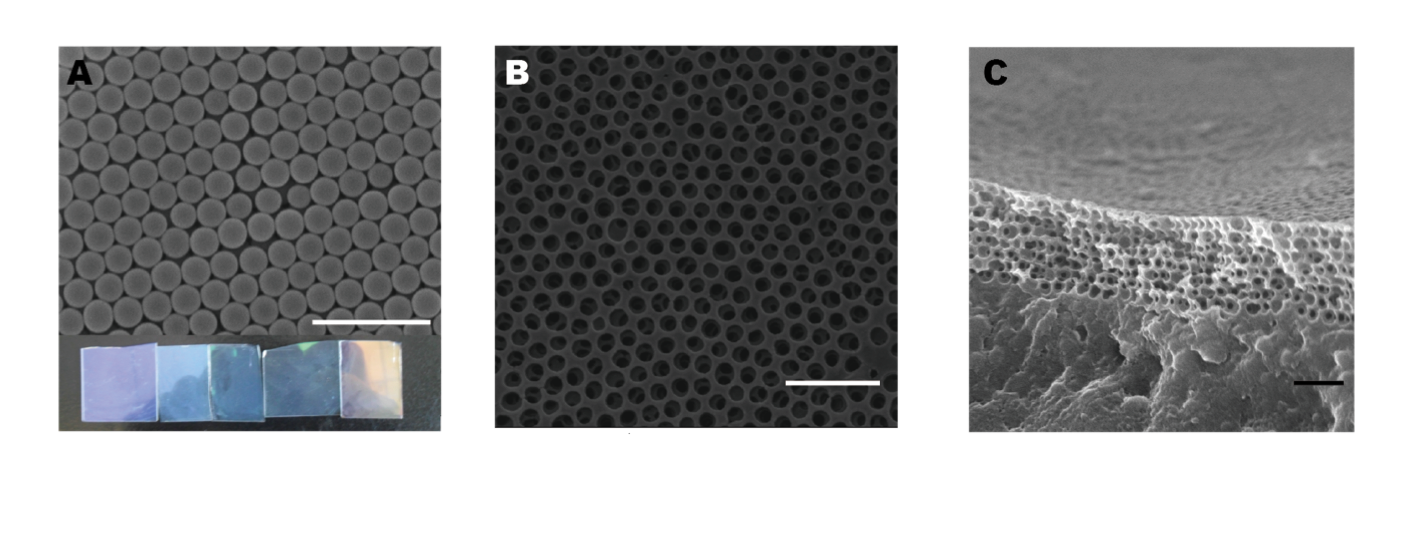
\includegraphics[width=\linewidth]{figures/ch2/mono-inverse.png}
  \caption{逐层堆积的SiO\text{$_2$}光子晶体制备反蛋白石模板。A. 逐层堆积的SiO\text{$_2$}模板与不同结构色的光子晶体的实物照片;B. 模板复制后的反蛋白石光子晶体SEM图;C. B图中反蛋白石光子晶体的剖面SEM照片。比例尺均为1 µm。}
  \label{fig:mono-inverse}
\end{figure}
同样使用PMMA作为反蛋白石材料的骨架,并使用HF刻蚀SiO\text{$_2$}。可以看出,采用逐层堆积法制备的反蛋白石光子晶体具有很好的孔道结构(图~\ref{fig:mono-inverse}B),
且由于逐层堆积的缘故,反蛋白石的表面较为平整,缺陷较少(图~\ref{fig:mono-inverse}C),说明逐层堆积法制备的三维光子晶体能够达到溶剂挥发诱导垂直沉积法光子晶体模板的质量。
同时,逐层堆积法制备的光子晶体模板面积较前者更大,能够很好地用于图案化光子晶体材料的制备。

\subsection{微流控液滴法制备SiO\text{$_2$}光子晶体模板}
\label{subsec:microfluid-opal}

前述两种方法均利用了胶体颗粒的组装过程制备了平面型的三维光子晶体模板材料。
本节中将基于微流控液滴技术来制备球形对称的光子晶体微球模板。
微流控液滴法的实质是利用含SiO\text{$_2$}胶体微球的液滴在加热挥发过程中胶体晶体自组装形成球形对称的光子晶体。
此方法中的液滴由同轴型微流控芯片制备,胶体微球的分散液作为微流控管道的内相,外相采用硅油(粘度10 cst)或十八烷等难于挥发的低密度有机溶剂。通过较快的外相液体的剪切作用将内相液体分散为粒径均等的液滴。通过调节内外相的相对流速大小可以对形成的液滴尺寸进行调控。
收集含有胶体微球液滴并在65-90 $^{\circ}$C条件下使液滴内水分挥发,诱导SiO\text{$_2$}收缩组装形成光子晶体微球。利用微流控液滴法制备SiO\text{$_2$}光子晶体微球的步骤具体如下:

1. 将干燥粉碎的SiO\text{$_2$}粉末在去离子水中充分超声分散,制备质量分数为20-30 \%的SiO\text{$_2$}分散液。通过如前所述的离心法(1000 rpm,2 min)去除无法分散的大块颗粒物。

2. 组装同轴微流控管道,并采用环氧树脂对其进行封闭,将微流控管道接入液体注射管道,并调节系统的水平度。后端采用PP材质的表面皿接收含胶体颗粒液滴的油相混合液。

3. 将微流控管道的注入端分别接入含SiO\text{$_2$}水相分散液及油相的微注射器,调节注射器旋进速度,使得后端接收的液滴间隔均匀,大小复合预期,此时可以开始接收所需的液滴。

4. 将流出液滴收集在表面皿中,,保持系统水平及稳定,防止水相液滴之间产生融合。当所需液滴收集数量满足要求之后,停止收集并将所有的接收表面皿放入65-90 $^{\circ}$C的烘箱中静置24h。此时原乳白色(胶体颗粒无定形排列)液滴产生明亮的结构色(胶体颗粒有序组装),组装即完成。

5. 将挥发形成的光子晶体微球收集于西林瓶中,去除油相溶剂,并利用石油醚或低沸点硅油(粘度0.1 cst)来洗涤残留的油相溶剂。将所得干燥的光子晶体微球置于马弗炉中600 $^{\circ}$C煅烧5 h,以增强光子晶体的机械强度。

微流控液滴的直径可以由两相液体的相对流速进行调控,通常在50-800 µm之间。经过水相挥发之后最终形成的光子晶体微球直径约收缩30-50\%,若水相胶体颗粒的质量分数过低时,形成的光子晶体微球收缩过大,容易造成结构不完整及光子晶体质量变差。一般采用20\%以上的质量分数以保证最终制备的光子晶体质量。
通过SEM照片可以看出(图~\ref{fig:ch2-CCB}B),
\begin{figure}[htbp]
  \centering
  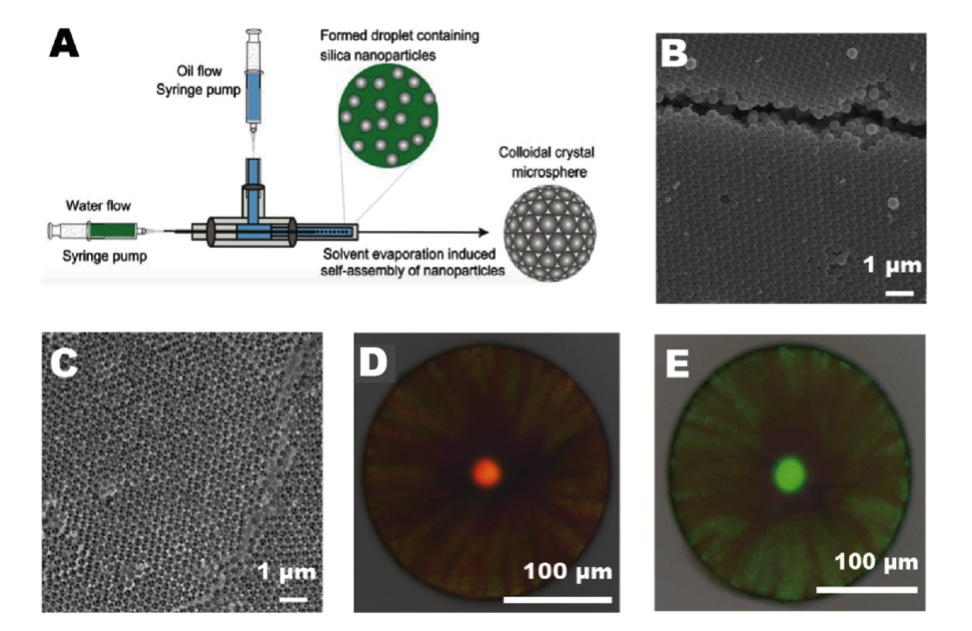
\includegraphics[width=\linewidth]{figures/ch2/CCB.png}
  \caption{微流控液滴制备法制备的SiO\text{$_2$}光子晶体微球及其反蛋白石模板。A. 微流控液滴制备法的原理示意图;B. SiO\text{$_2$}光子晶体微球的SEM图;C.反蛋白石光子晶体微球的SEM图。D、E分别为正模板与反蛋白石光子晶体微球的光学照片。}
  \label{fig:ch2-CCB}
\end{figure}
通过微流控液滴挥发制备的光子晶体微球中SiO\text{$_2$}颗粒呈现非常规整的fcc组装结构,且堆积紧密程度高于前述两种方法制备的光子晶体模板。与此对应的反蛋白石结构也具有相当高的结构规整性(图~\ref{fig:ch2-CCB}C)。
光学显微镜的观察可以发现其独特的光学结构,如图
  ~\ref{fig:ch2-CCB}D、\ref{fig:ch2-CCB}E
所示,这种球形的光子晶体存在一明显的中心亮斑,这是各方向反射的结构光汇聚后形成的。
由于中心亮斑的观测角度为垂直方向,因此其中心亮斑的Bragg衍射峰即代表了光子晶体微球内部排列的结构常数。此外,可以观察到围绕其中心亮斑也存在一些带状辐射的结构色带,这是由于球形的光子晶体造成的内部多晶衍射造成的。
同时,对其Bragg衍射峰的更加精细观察可以发现利用微流控液滴制备的光子晶体微球的Bragg衍射峰的半峰宽较窄(约30nm),小于前两种方法制备的光子晶体模板,应征了SEM中观察到的规整的SiO\text{$_2$}颗粒排列。

与平面型光子晶体模板制备反蛋白石结构的方法不同,球形对称的光子晶体微球模板不能利用三明治结构毛细作用法来填充聚合物前驱体;同时,由于聚合物在聚合过程中的体积收缩效应以及光子晶体微球中的重力作用,利用毛细作用预填充的光子晶体微球模板容易造成不对称的形貌,因此这里采用一种不同的方法来制作反蛋白石光子晶体微球,其步骤如下:

1. 将烧结后的SiO\text{$_2$}光子晶体微球置于平底的微型半密封容器中(易于取得的材料例如EP离心管的塑料封盖),将配置好的聚合物前驱液灌入其中。将容器平放入真空箱中处理1-2 min,直至光子晶体微球内部完全填充为止。

2. 将含预聚液的光子晶体微球置于聚合条件下(例如UV照射),直到聚合物充分固化。用工具刀将含光子晶体微球的聚合物块取出,并置于对该聚合物溶胀的溶剂中。例如,对于疏水的聚丙烯酸酯类聚合物,可选择氯仿作为溶胀溶剂。

3. 随着聚合物块溶胀并碎裂,部分光子晶体复合微球开始掉落;可采用超声以及机械力摩擦帮助光子晶体微球从聚合物块体中脱落。收集分离的光子晶体复合微球,并在显微镜下剔除形貌不规整的个体。

4. 将复合光子晶体微球从液相中分离干燥,并放入5 \% HF溶液中刻蚀,直到其中SiO\text{$_2$}被充分刻蚀为止(30 - 60 min)。至此即制备具有完整形貌的反蛋白石光子晶体微球。

这种制备光子晶体微球的方法主要利用了聚合物在溶剂中的溶胀作用。由于复合的微球中存在刚性的SiO\text{$_2$}颗粒(烧结后更加增加整体稳定性),因此在球形内部的聚合物膨胀受到局限;而外部的聚合物具有更大的体积膨胀。内外部的差别使得光子晶体微球能够弄聚合物块体中分离出来。
这种方法的另一个优点在于能够在光子晶体微球的表面形成完整的孔洞结构。SEM照片显示(图~\ref{fig:ch2-CCB}C),反蛋白石光子晶体微球的表面呈现出完整的六方排列的孔洞,而利用三明治结构制备的平面型光子晶体反蛋白石模板则容易由于表面不平整而使部分表面孔洞被覆盖。

结合上述实验,可以发现SiO\text{$_2$}光子晶体微球体现了与平面型光子晶体相似的光学与结构性质;同时,由于微流控液滴制备技术的引入,这种光子晶体微球材料具有制备速度快,重复性高、结构规整的优势,有望在实际应用中取代或提升平面型光子晶体材料。

\section{本章小结}

光子晶体模板材料的制备是光子晶体研究的基础。本章中对光子晶体模板制备方法进行了探究。
研究了Stöber方法制备SiO\text{$_2$}微粒,通过调节NH\text{$_3$}的浓度,实现了单分散SiO\text{$_2$}微粒粒径的调控。
利用这种方法制备的SiO\text{$_2$}微粒,结合胶体自组装方法,探究了三种光子晶体模板的制备方法。通过溶剂挥发诱导垂直沉积法制备了平面性的光子晶体模板,研究表明这种光子晶体模板具有规整的排列结构与光学特性。此外,为了改善大面积平面光子晶体模板的制备效率与大尺度完整性,我们发展了一种基于逐层堆积法的光子晶体模板制备方法,这种方法能够快速制备大面积的光子晶体材料,并且保持与溶剂挥发法同等的光子晶体质量。最后我们利用微流控液滴制备法制备了光子晶体微球模板材料,这种光子晶体模板较前两者具有更高的制备效率与重复性,且内部结构更为规整。通过上述探究,我们初步研究了光子晶体模板的制备方法,并将在随后的章节中使用本章中研究的光子晶体模板进行进一步的功能材料研究。

